\documentclass[man, 12pt, a4paper]{apa6}
\usepackage[american]{babel}
\usepackage{csquotes}
\usepackage[style=apa,sortcites=true,sorting=nyt,backend=biber]{biblatex}


\addbibresource{refs.bib}

\shorttitle{Norms and partner choice across settings}
\title{Title Goes Here}
\twoauthors{Sebastian Simon}{Jörg A. J. Gross}

\twoaffiliations{Faculty of Social, Economic and Behavioural Psychology,\linebreak Faculty of Social and Behavioural Sciences, Leiden University, the Netherlands}{Faculty of Social, Economic and Behavioural Psychology,\linebreak Faculty of Social and Behavioural Sciences, Leiden University, the Netherlands}

                    
%\abstract{}
%\keywords{}

\usepackage{caption}
\usepackage{subcaption}
\usepackage{graphicx}
\usepackage{wrapfig}


\begin{document}
%\parencites{}{}
%\citeauthor{}
%\citeyear{}
%\footcite[random comment]{}

\maketitle

Complex social norm systems are rules and standards that guide human behavior in groups (Cialdini, 2001; Pepitone, 1976) and are unique to humans (Tomasello and Rakoczy, 2003; Fehr and Rockenbach, 2004; Gintis, 2003; Ostrom, 2000; Sethi and Somanathan, 1996; Fehr and Fischbacher, 2003). Abiding to social norms is generally desirable (Hoffman, 1977; Freud, 1990) and doing so helps building and maintaining functional societies [ref]. For instance, in law and policy making … 

[example: law and policy making, EU]

Yet, people often choose to violate norms (Köbis, van Prooijen, Righetti, and Van Lange, 2016; Weisel and Shalvi, 2015) which, in turn, entails corrupt cooperation such as bribery (International Monetary Fund, 2016; Rose-Ackerman and Palifka, 2016), hindrance of economic growth (Mauro, 1995), and undermining of the legitimacy and capacity of governments (Rothstein, 2011). For instance, corrupt police entities cooperating with drug cartels … 

[example: drug cartels]

Here we argue that cooperation is not prosocial per se but depends on a) the possibility to choose viable interaction partners, b) the incentive structures of the settings people are in, and c) the order of these settings. 

Previous research highlighted the importance of interpersonal variables in predicting cooperation through morality goals. As people like to think of themselves as moral beings (Bazar, Amir, and Ariely, 2008; Jordan, Mullen, and Nurninghan, 2011; Abeler, Becker, and Falk, 2014; Abeler, Nosenzo, and Raymond, 2016) and care about what others think of them (Lacetera and Macis, 2010; Utikal and Fischbacker, 2013; Gausel and Leach, 2011), moral traits dominate [abele and wojciszke, 2014; cottrell, neuberg li, 2007; landy, piazza, Goodwin, 2016; landy, uhlmann, 2016; peeters, 1992, wojciszke, abele, baryla, 2009]. For instance, we prefer to interact with those who are warm and sociable, competent and capable [ref]. 


\section{Social Norms}

Most of the time, I got to the institute by foot, bike, and train and worked from there. The remaining time, I either worked from outside the institute or from home (see section Working at Conferences). In my opinion, reporting merely on my activities and their processes does not capture my entire learning experience. So, I will discuss the work environment first and then proceed to what I did during my internship.  

\section{Partner Choice} 
 
\subsection{The Team and Environment}

There are five theme groups at NiDi and all of them are differently structured according to their projects. For instance, I got accepted for a research internship at the \textit{Gender and Generations Programme (GGP)} which is part of the \textit{Families and Generations} theme group. 

\begin{wrapfigure}{r}{0.55\textwidth}
  \vspace{-30pt}
  \begin{center}
    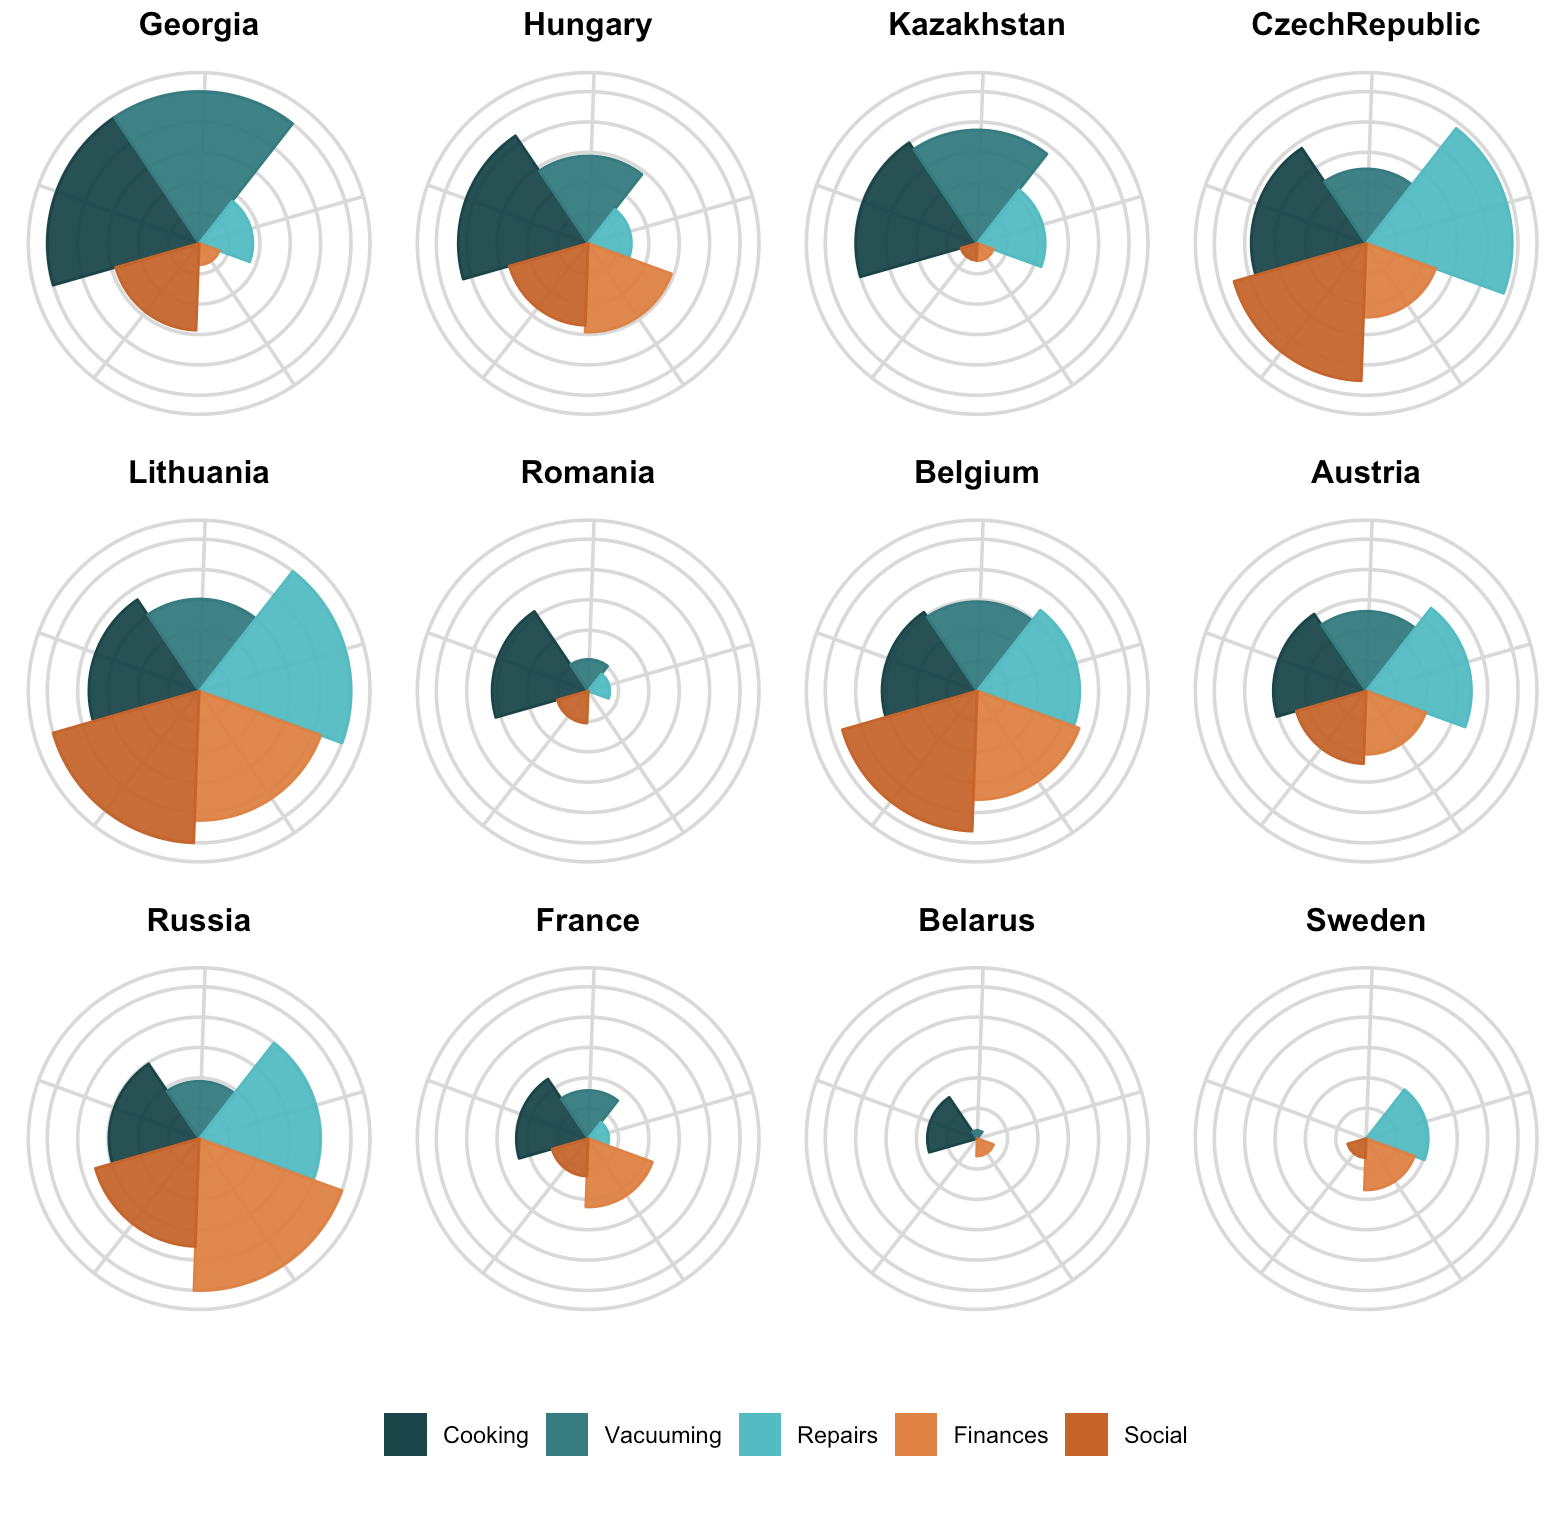
\includegraphics[width=0.6\textwidth]{Nightingale}
  \end{center}
  \vspace{-30pt}
  \caption{Nightingale plots showing how equal women perceived the household tasks to be distributed among them and their partners.}
\end{wrapfigure}

\printbibliography

% I have commented out the appendix section since it isn't a standard for minimal documents. 
%\appendix \usepackage{•} 

\end{document}


